% Rapport de stage -- Projet de prevision de la demande electrique
% Compiler avec: pdflatex rapport_stage_mogador.tex (deux fois)
\documentclass[12pt,a4paper,oneside]{report}

\usepackage[T1]{fontenc}
\usepackage[utf8]{inputenc}
\usepackage[french]{babel}
\usepackage{lmodern}
\usepackage{geometry}
\usepackage{graphicx}
\usepackage{xcolor}
\usepackage{booktabs}
\usepackage{array}
\usepackage{longtable}
\usepackage{amsmath}
\usepackage{hyperref}
\usepackage{enumitem}
\usepackage{float}
\usepackage{caption}
\geometry{left=3cm,right=2.5cm,top=2.5cm,bottom=2.5cm}
\hypersetup{colorlinks=true,linkcolor=blue,urlcolor=blue,citecolor=blue}
\setlength{\parskip}{0.45em}
\setlength{\parindent}{0pt}
\setlength{\emergencystretch}{3em}

% ---------- Informations a personnaliser ----------
\newcommand{\Etablissement}{\textbf{[Nom de l'ecole ou universite]}}
\newcommand{\Filiere}{\textbf{[Filiere et option]}}
\newcommand{\Etudiant}{\textbf{[Nom et prenom de l'etudiant]}}
\newcommand{\Annee}{\textbf{[Annee universitaire]}}
\newcommand{\Periode}{\textbf{[Periode du stage]}}
\newcommand{\EncadrantEcole}{\textbf{[Nom de l'encadrant pedagogique]}}
\newcommand{\EncadrantEntreprise}{\textbf{[Nom de l'encadrant MOGADOR TECHNOLOGIE INDUSTRIELLE]}}

% Reserve une zone visible pour une capture ou un diagramme.
\newcommand{\visualplaceholder}[3]{%
  \begin{figure}[H]
  \centering
  \fbox{\begin{minipage}[c][#2][c]{0.88\textwidth}\centering
  \textit{Emplacement reserve : #1}\\[0.5em]
  \small Inserer le fichier final ici avec \texttt{\textbackslash includegraphics}.
  \end{minipage}}
  \caption{#3}
  \end{figure}}

\begin{document}

% ---------- Page de garde ----------
\begin{titlepage}
\centering
\vspace*{1cm}
\Etablissement\\[0.4cm]
\Filiere\\[1.2cm]
\fbox{\parbox[c][2.3cm][c]{5cm}{\centering \small Logo de l'etablissement}}\hfill
\fbox{\parbox[c][2.3cm][c]{5cm}{\centering \small Logo MOGADOR TECHNOLOGIE INDUSTRIELLE}}\\[1.6cm]
{\Large \textbf{RAPPORT DE STAGE}}\\[0.5cm]
{\LARGE \textbf{Prevision horaire de la demande electrique}}\\[0.3cm]
{\large Conception d'une application de prevision et de suivi de qualite des donnees}\\[1.2cm]
\begin{tabular}{@{}>{\raggedright\arraybackslash\bfseries}p{5cm}>{\raggedright\arraybackslash}p{8.4cm}@{}}
Realise par : & \Etudiant\\[0.25cm]
Entreprise d'accueil : & \textbf{MOGADOR TECHNOLOGIE INDUSTRIELLE}\\[0.25cm]
Periode : & \Periode\\[0.25cm]
Encadrant pedagogique : & \EncadrantEcole\\[0.25cm]
Encadrant entreprise : & \EncadrantEntreprise\\[0.25cm]
Annee universitaire : & \Annee
\end{tabular}
\vfill
\textit{Document a completer avec les informations administratives validees par MOGADOR TECHNOLOGIE INDUSTRIELLE et l'etablissement.}
\end{titlepage}

\chapter*{Remerciements}
\addcontentsline{toc}{chapter}{Remerciements}
Je remercie la direction de MOGADOR TECHNOLOGIE INDUSTRIELLE pour l'accueil et l'opportunite de realiser ce stage. J'adresse mes remerciements particuliers a mon encadrant en entreprise, a mon encadrant pedagogique et a toutes les personnes ayant contribue aux echanges metier et techniques. Leur accompagnement a permis de transformer un besoin de pilotage de la consommation electrique en une solution logicielle structuree et verifiable.

\chapter*{Resume}
\addcontentsline{toc}{chapter}{Resume}
Ce rapport presente la conception et la realisation d'une application de prevision horaire de la demande electrique dans le cadre d'un stage chez MOGADOR. La solution combine un modele XGBoost, des variables calendaires, des retards de demande et des donnees meteorologiques. Elle expose ses resultats au moyen d'une API FastAPI et d'une interface React. Le travail ne se limite pas a la prediction : il introduit un contrat d'ingestion pour les donnees reelles, des controles de qualite, une evaluation separee entre prediction a un pas et prevision recursive, des intervalles d'incertitude estimes, ainsi qu'un processus de reentrainement protege.

Les resultats disponibles proviennent du jeu de donnees synthetique inclus dans le projet. Sur la periode de test 2024 tenue a l'ecart, le modele XGBoost actif atteint une WAPE de 3,55\% et une RMSE de 130,22 MW. Ces mesures constituent une demonstration technique et ne doivent pas etre interpretees comme des performances operationnelles avant validation sur des donnees reelles de MOGADOR.

\textbf{Mots-cles :} prevision de charge, XGBoost, donnees horaires, FastAPI, React, qualite des donnees, incertitude.

\chapter*{Abstract}
\addcontentsline{toc}{chapter}{Abstract}
This report presents the design and implementation of an hourly electricity-demand forecasting application developed during an internship at MOGADOR. The solution combines an XGBoost model with calendar variables, demand lags and weather data. A FastAPI backend and a React interface make forecasts and evaluation results accessible. The project also establishes a local real-data ingestion contract, data-quality checks, separate one-step and recursive evaluations, estimated uncertainty intervals and a safeguarded retraining workflow.

The available results are based on the project's synthetic dataset. On the untouched 2024 test period, the active XGBoost model reaches a 3.55\% WAPE and a 130.22 MW RMSE. These values demonstrate the technical workflow only and require validation on real MOGADOR data before operational use.

\textbf{Keywords:} load forecasting, XGBoost, hourly data, FastAPI, React, data quality, uncertainty.

\tableofcontents
\listoffigures
\listoftables

\chapter*{Liste des abreviations}
\addcontentsline{toc}{chapter}{Liste des abreviations}
\begin{longtable}{p{3cm}p{10cm}}
API & Application Programming Interface, interface de programmation applicative.\\
MAE & Mean Absolute Error, erreur absolue moyenne.\\
RMSE & Root Mean Squared Error, racine de l'erreur quadratique moyenne.\\
WAPE & Weighted Absolute Percentage Error, erreur absolue ponderee en pourcentage.\\
XGBoost & Extreme Gradient Boosting, methode d'apprentissage par arbres de decision.\\
\end{longtable}

\chapter*{Introduction generale}
\addcontentsline{toc}{chapter}{Introduction generale}
La consommation electrique varie selon l'heure, le jour, la saison, la meteo et les habitudes d'exploitation. Une estimation fiable de la demande permet de mieux planifier les ressources, d'anticiper les pointes et d'appuyer les decisions de pilotage. Dans ce contexte, le stage chez MOGADOR porte sur la mise en place d'un prototype de prevision horaire de la demande electrique, exploitable a travers une interface web locale.

La problematique est la suivante : comment construire une chaine de prevision qui produise des resultats interpretable, tout en rendant visibles la qualite des donnees, les limites du modele et les conditions necessaires a une utilisation sur des donnees reelles ? Les objectifs sont de concevoir un modele de reference robuste, de proposer une API et un tableau de bord, et de preparer le projet a l'integration future de flux reels de demande et de meteo.

Le premier chapitre presente le contexte et les besoins. Le deuxieme etudie les choix technologiques. Le troisieme decrit l'architecture et le pipeline de donnees. Le quatrieme detaille l'implementation et les tests. Enfin, le cinquieme analyse les resultats, les limites et les perspectives.

\chapter{Contexte et cahier des charges}
\section{Presentation de l'entreprise d'accueil}
MOGADOR TECHNOLOGIE INDUSTRIELLE est l'entreprise d'accueil du stage. Cette section doit etre completee a partir d'informations institutionnelles validees : secteur d'activite, organisation, missions, site d'accueil et service de rattachement. Il est important de ne pas ajouter de chiffres, de clients ou de projets non confirmes.

\visualplaceholder{Presentation de MOGADOR TECHNOLOGIE INDUSTRIELLE : logo, organigramme ou photographie autorisee}{5cm}{Presentation de l'entreprise d'accueil}

\section{Contexte metier et problematique}
Le projet traite la prevision de charge electrique a une granularite horaire. Une prediction calculee a l'avance peut aider a identifier les periodes de forte demande et a mettre a disposition des indicateurs de suivi. Cependant, une prediction n'est exploitable que si les donnees utilisees sont identifiees, completes et compatibles avec le modele.

\section{Analyse de l'existant}
Le point de depart est un prototype de prevision base sur un jeu de donnees local. La version initiale permettait la consultation de donnees historiques et de predictions. Les principaux axes d'amelioration identifies sont l'explicitation du caractere synthetique des donnees, la formalisation d'un format d'ingestion, la distinction entre meteo observee et meteo future, et la mise en evidence des limites de la prevision multi-horizon.

\section{Expression des besoins}
\subsection{Besoins fonctionnels}
\begin{itemize}[leftmargin=*]
\item Charger localement des donnees horaires de demande, temperature et humidite au format CSV ou XLSX.
\item Consulter des statistiques, une analyse de demande, des predictions historiques et des previsions futures.
\item Visualiser la qualite des donnees : doublons, trous horaires, valeurs manquantes, valeurs atypiques et couverture temporelle.
\item Afficher les performances par horizon et des intervalles de prediction estimes.
\item Conserver les artefacts candidats lors d'un reentrainement et ne promouvoir un modele que s'il ameliore le test tenu a l'ecart.
\end{itemize}
\subsection{Besoins non fonctionnels}
La solution doit etre locale, reproductible, testable et explicite sur ses hypotheses. Aucun secret ne doit etre code en dur. Les donnees reelles et les previsions meteorologiques externes ne doivent pas etre inventees ni telechargees sans configuration explicite.

\chapter{Etat de l'art et choix technologiques}
\section{Prevision de la demande electrique}
Les methodes de prevision incluent les approches naives, les modeles statistiques de series temporelles et les methodes d'apprentissage automatique. Dans ce projet, les baselines a 24 heures et 168 heures servent de points de comparaison. Elles reproduisent respectivement la charge du jour precedent et de la semaine precedente.

Les arbres de decision par gradient boosting sont pertinents lorsque les variables explicatives combinent calendrier, meteo et retards de demande. XGBoost a ete retenu car il gere les relations non lineaires, fournit une importance des variables et s'integre simplement a un pipeline Python.

\begin{table}[H]
\centering
\caption{Comparaison qualitative des approches envisagees}
\begin{tabular}{>{\raggedright\arraybackslash}p{3cm}>{\raggedright\arraybackslash}p{3cm}>{\raggedright\arraybackslash}p{3cm}>{\raggedright\arraybackslash}p{3cm}}
\toprule
Approche & Atout & Limite & Decision\\
\midrule
Naive 24h / 168h & Tres interpretable, rapide & Ne capture pas les variations complexes & Baseline\\
ARIMA/SARIMA & Base statistique connue & Parametrage delicat avec plusieurs variables & Non retenue pour le prototype\\
Reseau LSTM & Peut modeliser des sequences longues & Besoin de plus de donnees et de reglages & Non retenue a ce stade\\
XGBoost & Efficace sur variables tabulaires, interpretable & Prevision recursive sensible a l'accumulation d'erreurs & Retenue\\
\bottomrule
\end{tabular}
\end{table}

\section{Technologies retenues}
Le backend est developpe avec Python, Pandas, XGBoost et FastAPI. Le frontend utilise React et Vite. Les tests backend sont executes avec Pytest et les tests frontend avec Vitest. Cette separation facilite la reutilisation des fonctions de caracteristiques et d'evaluation entre l'API, les tests et le processus de reentrainement.

\chapter{Conception et architecture}
\section{Methodologie de travail}
Le travail est organise en iterations courtes : analyse du comportement existant, ajout d'une amelioration, creation de tests cibles, puis verification du build. Cette approche convient a un prototype logiciel car elle limite les regressions et conserve une trace des decisions techniques.

\section{Architecture globale}
L'application comporte trois couches. La couche donnees lit les fichiers locaux et applique les controles de qualite. La couche metier construit les variables causales, effectue les predictions et calcule les metriques. La couche presentation expose les resultats via FastAPI et React.

\visualplaceholder{Diagramme d'architecture : fichiers locaux, backend FastAPI, modele XGBoost, frontend React}{6cm}{Architecture fonctionnelle de la solution}

\section{Pipeline de donnees et caracteristiques}
Les colonnes requises sont \texttt{Timestamp}, \texttt{Demand}, \texttt{Temperature} et \texttt{Humidity}. Les observations doivent etre horaires. Les controles detectent les doublons, les lacunes, les valeurs manquantes et les valeurs atypiques. La meteo peut etre propagee uniquement vers l'avant pour eviter d'utiliser une information future. La demande n'est pas imputee comme cible ; elle est uniquement propagee dans l'historique causal necessaire aux retards.

Les variables incluent l'heure, le jour de semaine, le mois, des encodages cycliques, les jours feries, la temperature, son carre, des retards de 1 a 336 heures et des statistiques glissantes. Cette construction assure que les variables de demande utilisees pour une heure donnee proviennent strictement du passe.

\visualplaceholder{Schema du pipeline : ingestion, validation, features, modele, API et interface}{6cm}{Pipeline de traitement et de prevision}

\section{Evaluation et incertitude}
Les performances a un pas utilisent les retards et la meteo observes. Les performances multi-pas sont calculees en mode recursif : une prediction peut alimenter les retards suivants. Les deux types de resultats sont presentes separement pour eviter une interpretation abusive.

Un intervalle empirique a 90\% est construit a partir des residus absolus du jeu de test. Pour les horizons recursifs, son rayon augmente suivant une regle en racine de l'horizon. Cet intervalle est une estimation et non une garantie de couverture.

\chapter{Realisation et implementation}
\section{Environnement de developpement}
Le projet est organise autour des dossiers \texttt{backend}, \texttt{frontend}, \texttt{data} et \texttt{models}. FastAPI fournit les endpoints REST ; React affiche les pages Apercu, Analyse de la demande, Performance du modele et Prevision. Les pages de graphiques sont chargees a la demande pour reduire le poids initial du frontend.

\section{Contrat d'ingestion des donnees reelles}
La variable d'environnement \texttt{ELECTRICITY\_DATA\_PATH} indique un fichier local CSV, XLSX ou XLS. La variable \texttt{WEATHER\_FORECAST\_PATH} peut pointer vers un fichier local de previsions meteorologiques contenant \texttt{Timestamp}, \texttt{Temperature} et \texttt{Humidity}. Sans fichier configure, l'application utilise un proxy historique explicitement affiche comme tel. Les evenements non publics sont ajoutes uniquement depuis un fichier verifie, configure avec \texttt{VERIFIED\_EVENTS\_PATH} et contenant \texttt{Date} et \texttt{Event}.

\begin{figure}[H]
\centering
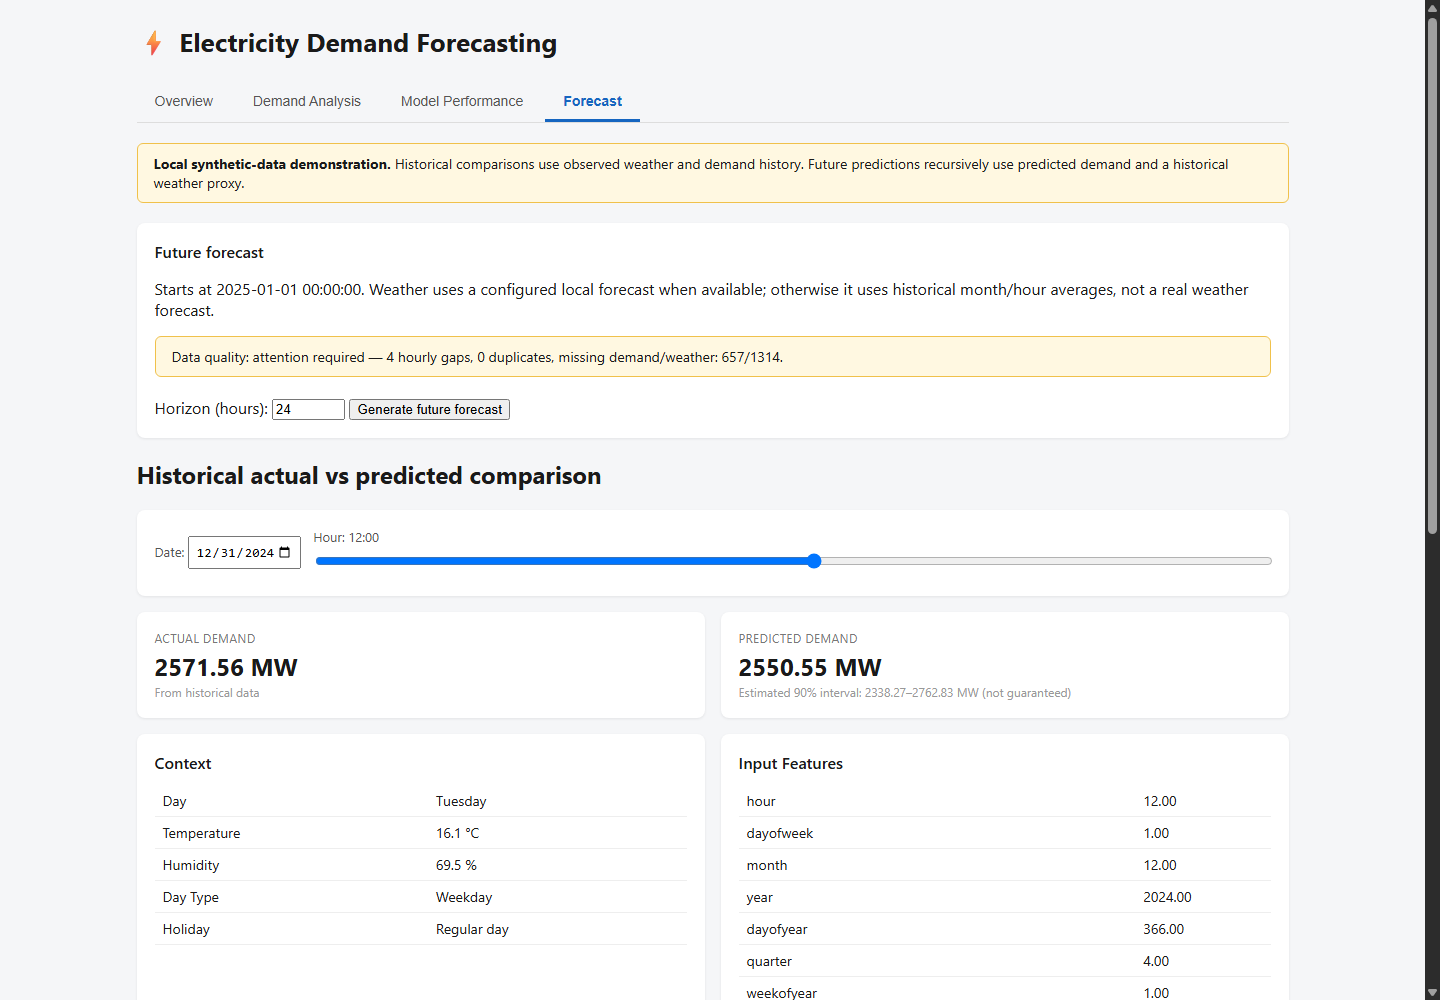
\includegraphics[width=0.93\textwidth]{figures/capture_prevision.png}
\caption{Interface de prevision future executee localement}
\end{figure}

\section{Workflow de reentrainement protege}
Le reentrainement est volontairement manuel. La commande suivante refuse le jeu synthetique integre :
\begin{center}
\small\texttt{python -m backend.modeling --train --data}\\
\texttt{chemin\_vers\_donnees\_reelles.csv}
\end{center}
Elle conserve un artefact candidat, emploie des validations chronologiques et compare le candidat au modele actif sur le holdout 2024. La promotion n'est realisee que si la WAPE ou la RMSE s'ameliore strictement sur les memes lignes valides.

\section{Tests}
Les tests verifient les caracteristiques causales, les validations de l'API, la prevision recursive, les metriques, le contrat d'ingestion, la qualite des donnees et l'affichage frontend. La verification finale comprend les tests Pytest, les tests Vitest et la construction du frontend avec Vite.

\visualplaceholder{Capture du terminal montrant les tests Pytest, Vitest et le build Vite}{5cm}{Verification automatisee du projet}

\chapter{Resultats et discussion}
\section{Resultats sur le jeu de demonstration}
Le modele XGBoost actif a ete evalue sur une periode de test 2024 non utilisee pendant l'entrainement ni l'arret anticipe. Le tableau \ref{tab:resultats} reprend les indicateurs documentes dans le projet. Les valeurs sont liees au jeu de demonstration synthetique.

\begin{table}[H]
\centering
\caption{Resultats sur le holdout synthetique 2024}
\label{tab:resultats}
\begin{tabular}{lrrrr}
\toprule
Modele & MAE (MW) & RMSE (MW) & R$^2$ & WAPE (\%)\\
\midrule
Naive 24 heures & 178,25 & 224,53 & 0,7860 & 6,09\\
Naive 168 heures & 144,33 & 181,99 & 0,8594 & 4,93\\
XGBoost precedent & 112,95 & 141,32 & 0,9152 & 3,86\\
XGBoost actif & \textbf{103,72} & \textbf{130,22} & \textbf{0,9280} & \textbf{3,55}\\
\bottomrule
\end{tabular}
\end{table}

Ces resultats montrent une amelioration par rapport aux baselines et a l'ancien modele dans le cadre du jeu synthetique. Ils ne valident pas encore une utilisation en production chez MOGADOR. La validation operationnelle necessite des donnees historiques reelles, un referentiel de fuseau horaire confirme et des previsions meteorologiques disponibles au moment de la prediction.

\begin{figure}[H]
\centering
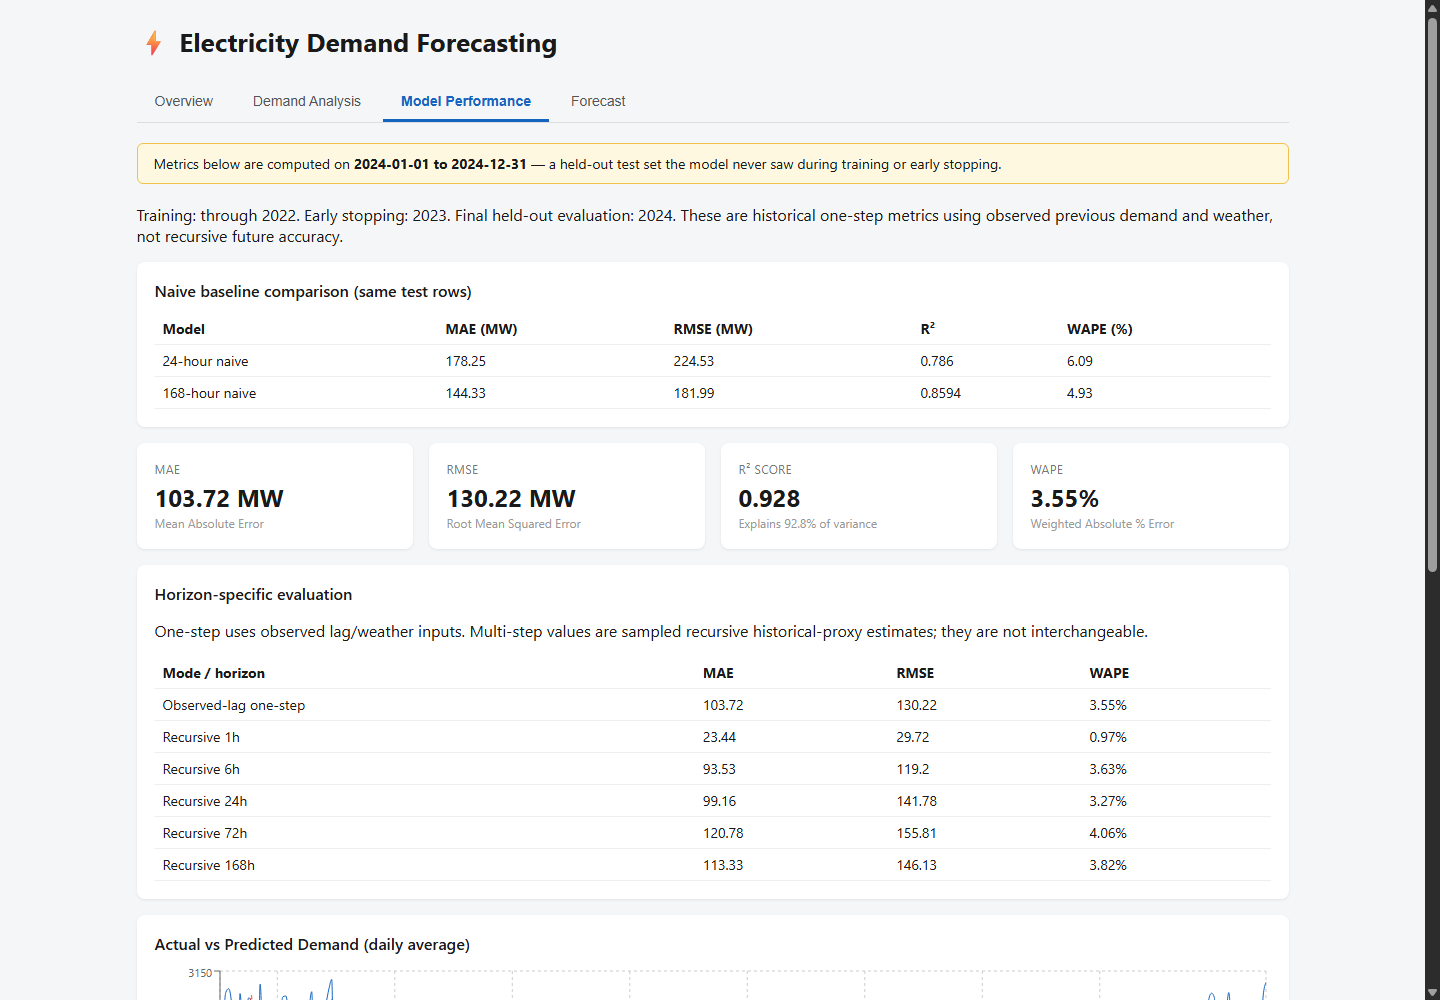
\includegraphics[width=0.93\textwidth]{figures/capture_performance_modele.png}
\caption{Performances du modele, baselines et horizons sur le holdout}
\end{figure}

\section{Limites identifiees}
La principale limite est l'absence de donnees operationnelles reelles dans le depot. Les valeurs de meteo futures peuvent etre fournies par fichier, mais aucun fournisseur externe n'est branche sans identifiants. Enfin, les previsions recursives accumulent des erreurs a mesure que l'horizon augmente. Les intervalles affiches doivent donc etre lus comme des estimations empiriques et non comme des garanties.

\chapter*{Conclusion generale et perspectives}
\addcontentsline{toc}{chapter}{Conclusion generale et perspectives}
Le stage a abouti a une application locale de prevision de demande electrique fondee sur XGBoost. La solution fournit une interface web, une API, des metriques de test et des mecanismes qui preparent l'integration de donnees reelles : contrat d'ingestion, controles de qualite, gestion explicite de la meteo future, intervalles estimes et reentrainement protege.

Les prochaines etapes sont l'obtention et la validation de donnees reelles de MOGADOR, la definition d'un protocole de mise a jour des donnees, l'integration d'une source meteorologique autorisee, l'ajout de variables metier verifiees et l'evaluation continue des performances par horizon. Une comparaison avec des modeles probabilistes ou des approches de prevision directe par horizon pourra egalement etre etudiee.

\begin{thebibliography}{9}
\bibitem{xgboost} T. Chen et C. Guestrin, ``XGBoost: A Scalable Tree Boosting System'', Proceedings of KDD, 2016.
\bibitem{fastapi} FastAPI, ``FastAPI Documentation''. \url{https://fastapi.tiangolo.com/}.
\bibitem{react} React, ``React Documentation''. \url{https://react.dev/}.
\bibitem{project} Documentation interne du projet, \texttt{README.md}, consultee dans le depot local.
\end{thebibliography}

\appendix
\chapter{Guide d'insertion des captures et diagrammes}
Chaque encadre du rapport est une zone reservee. Remplacer, par exemple, un appel a \texttt{\textbackslash visualplaceholder} par :
\begin{verbatim}
\begin{figure}[H]
  \centering
  \includegraphics[width=0.88\textwidth]{figures/nom-de-la-capture.png}
  \caption{Description precise de la capture}
  \label{fig:nom-capture}
\end{figure}
\end{verbatim}
Creer un dossier \texttt{figures} a cote de ce fichier \LaTeX{} et utiliser des images autorisees par MOGADOR. Pour les diagrammes, privilegier des exports PDF ou PNG lisibles.

\chapter{Commandes de verification}
\begin{verbatim}
python -m pytest backend/tests -q
cd frontend
npm exec vitest run
npm run build
\end{verbatim}

% Annexes detaillees : chaque section commence sur une nouvelle page.
\clearpage
\section{Vue generale de l'application}
\begin{figure}[H]\centering
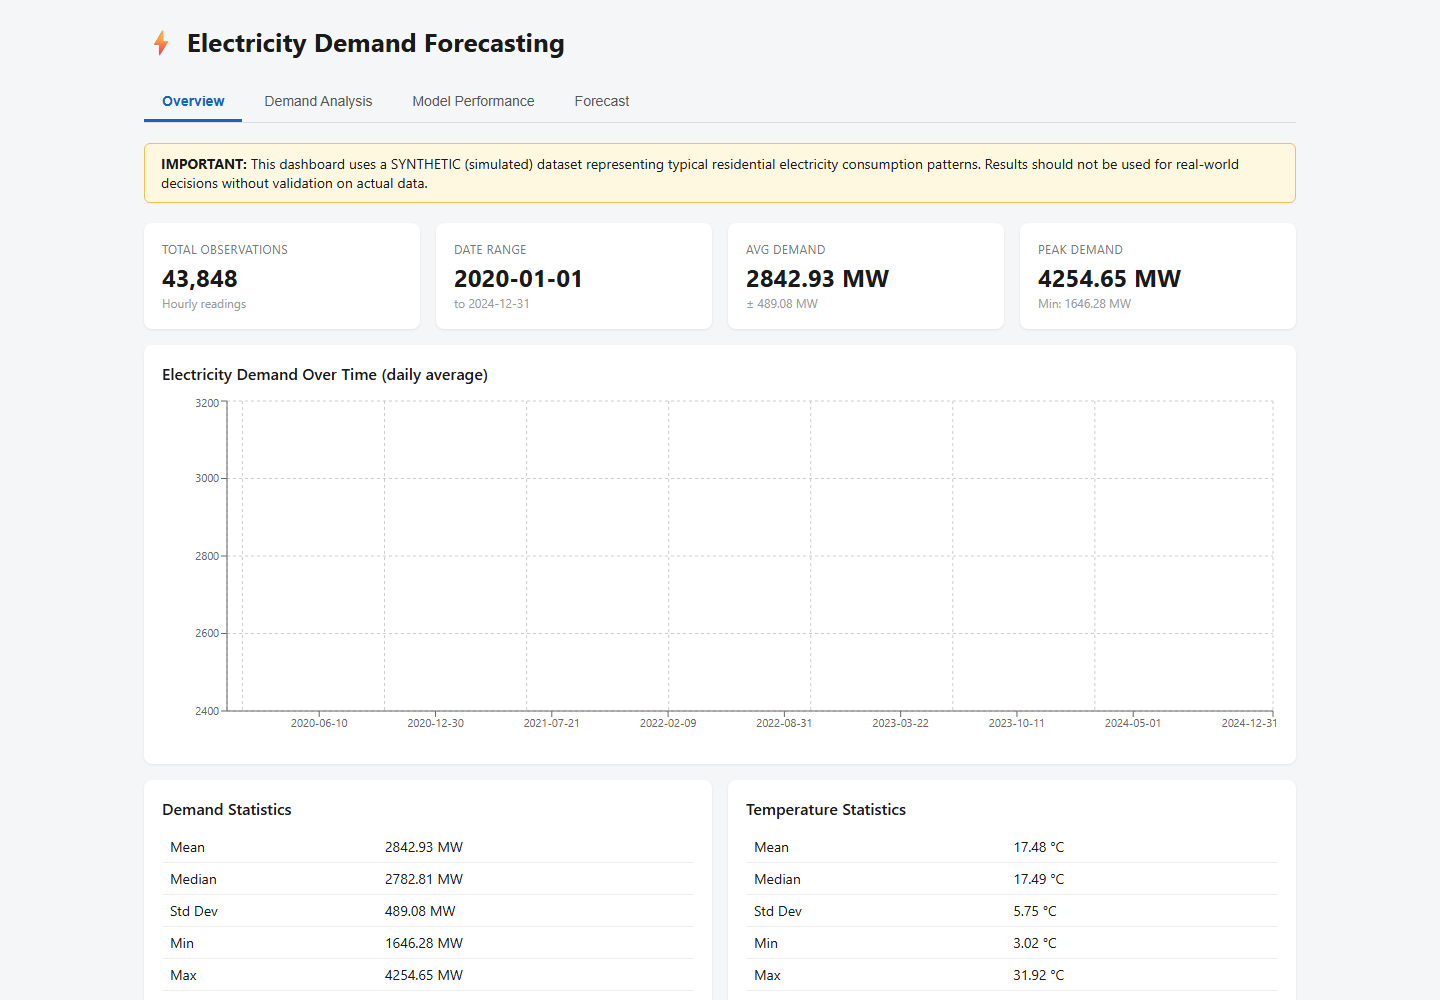
\includegraphics[width=0.95\textwidth]{figures/capture_vue_ensemble.png}
\caption{Vue generale de l'application locale et avertissement sur les donnees synthetiques}
\end{figure}
La page d'accueil rassemble le nombre d'observations, la plage temporelle, la demande moyenne, le pic et les statistiques meteorologiques. La banniere rappelle que le jeu courant est simule. Cette information doit rester visible avant toute interpretation des graphiques.

\clearpage
\section{Documentation interactive de l'API}
\begin{figure}[H]\centering
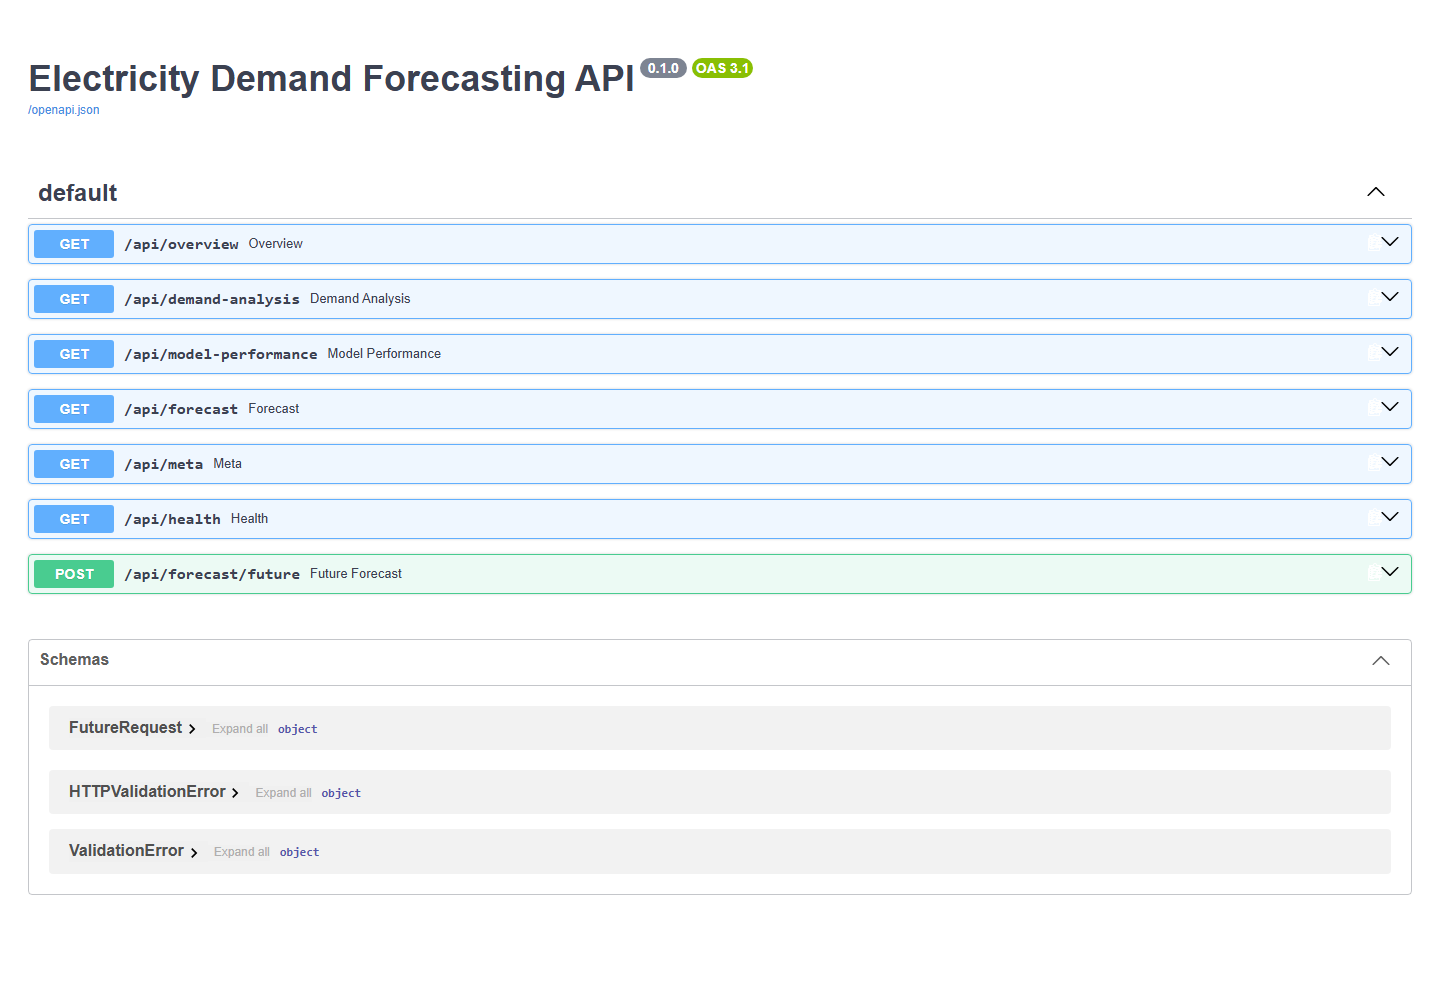
\includegraphics[width=0.95\textwidth]{figures/capture_api_fastapi.png}
\caption{Documentation OpenAPI generee automatiquement par FastAPI}
\end{figure}
L'interface Swagger enumere les routes de synthese, d'analyse, de performance, de sante et de prevision. Elle permet de verifier le contrat sans passer par React. Le schema \texttt{FutureRequest} documente le debut, l'horizon et les tableaux meteorologiques optionnels.

\clearpage
\section{Diagramme des cas d'utilisation}
\visualplaceholder{Diagramme UML : consulter, analyser, prevoir, controler et reentrainer}{12cm}{Cas d'utilisation de la plateforme}
Acteurs proposes : utilisateur metier, analyste data et administrateur technique. Relier chaque acteur uniquement aux actions effectivement autorisees par MOGADOR TECHNOLOGIE INDUSTRIELLE.

\clearpage
\section{Diagramme de sequence}
\visualplaceholder{Sequence entre React, FastAPI, meteo, features et XGBoost}{12cm}{Sequence de la prevision future}
Faire apparaitre la validation de l'horizon, le choix entre meteo fournie et proxy, la boucle recursive et la construction des intervalles. Ajouter un chemin d'erreur pour une couverture meteorologique incomplete.

\clearpage
\section{Diagramme de composants}
\visualplaceholder{Composants backend, frontend, artefacts, fichiers et tests}{12cm}{Organisation des composants logiciels}
Le diagramme peut suivre les dossiers du depot. Il doit distinguer les dependances d'execution de celles de developpement et montrer le partage des fonctions de caracteristiques entre entrainement et inference.

\clearpage
\section{Diagramme de deploiement local}
\visualplaceholder{Poste local, navigateur, Vite, Uvicorn et stockage local}{12cm}{Deploiement actuel de la solution}
Le navigateur contacte Vite sur le port 5173 et FastAPI sur le port 8000. Les fichiers de donnees et de modele restent sur la machine. Aucune ressource cloud n'est necessaire dans le perimetre actuel.

\clearpage
\section{Dictionnaire de la table historique}
\begin{longtable}{p{3.2cm}p{3cm}p{7cm}}
\toprule Champ & Type attendu & Regle\\\midrule
Timestamp & Date-heure & Une valeur par heure, sans doublon\\
Demand & Numerique & Demande cible en MW\\
Temperature & Numerique & Unite homogene et documentee\\
Humidity & Numerique & Pourcentage de 0 a 100\\
\bottomrule
\end{longtable}
Les colonnes additionnelles sont tolerees mais ignorees par le chargeur canonique. Toute unite differente doit etre convertie avant utilisation et tracee dans la documentation de la source.

\clearpage
\section{Caracteristiques calendaires}
Les variables \texttt{hour}, \texttt{dayofweek}, \texttt{month}, \texttt{year}, \texttt{dayofyear}, \texttt{quarter} et \texttt{weekofyear} decrivent la position d'une observation. Les couples sinus/cosinus representent la continuite entre 23 h et 0 h ou entre dimanche et lundi. Les indicateurs \texttt{is\_weekend} et \texttt{is\_holiday} isolent des regimes particuliers. Les jours feries viennent de la bibliotheque et les evenements internes d'un fichier verifie.

\clearpage
\section{Retards et fenetres glissantes}
Les retards de 1, 2, 3, 6 et 12 heures capturent la dynamique intrajournaliere. Ceux de 24, 48 et 72 heures representent les repetitions quotidiennes. Les retards de 168 et 336 heures correspondent a une et deux semaines. Les moyennes et ecarts-types glissants sur 6, 24 et 168 heures mesurent le niveau et la variabilite recents. Toutes ces variables sont calculees apres un decalage causal.

\clearpage
\section{Exemple de fichier de donnees reelles}
\begin{verbatim}
Timestamp,Demand,Temperature,Humidity
2026-01-01 00:00:00,<demande>,<temperature>,<humidite>
2026-01-01 01:00:00,<demande>,<temperature>,<humidite>
\end{verbatim}
Cet extrait illustre seulement la structure. Les chevrons doivent etre remplaces par des mesures validees. Le fichier doit etre continu a l'heure, employer un fuseau confirme et conserver des unites constantes. La source, la date d'extraction et le responsable doivent etre documentes.

\clearpage
\section{Exemple de fichier meteorologique futur}
\begin{verbatim}
Timestamp,Temperature,Humidity
2026-01-02 00:00:00,<temperature prévue>,<humidite prévue>
2026-01-02 01:00:00,<temperature prévue>,<humidite prévue>
\end{verbatim}
Le fichier doit couvrir chaque heure demandee. Une seule lacune provoque un refus afin d'eviter le melange silencieux d'une vraie prevision et d'un proxy. Le fournisseur, l'heure d'emission et l'horizon du bulletin devront etre traces.

\clearpage
\section{Exemple de fichier d'evenements verifies}
\begin{verbatim}
Date,Event
<date validee>,<nom de l'evenement valide>
\end{verbatim}
Aucune date interne n'est pre-remplie. Les evenements doivent etre connus au moment de la prevision. Un identifiant, une categorie, une heure de debut, une heure de fin et un perimetre pourront completer le schema apres validation metier.

\clearpage
\section{Catalogue des controles de qualite}
\begin{tabular}{p{4cm}p{5cm}p{5cm}}
\toprule Controle & Detection & Traitement\\\midrule
Doublon & Timestamp repete & Statut incompatible\\
Trou horaire & Grille attendue & Nombre et premier trou\\
Valeur manquante & Valeur nulle & Comptage par variable\\
Valeur atypique & Trois IQR & Signalement uniquement\\
Couverture & Min et max & Exposition API\\
Historique & Longueur requise & Refus si insuffisant\\
\bottomrule
\end{tabular}
Une anomalie doit etre examinee avec son contexte. Un seuil ne distingue pas automatiquement une erreur de capteur d'un evenement industriel reel.

\clearpage
\section{Catalogue des endpoints}
\begin{longtable}{p{4cm}p{2cm}p{7cm}}
\toprule Route & Methode & Finalite\\\midrule
/api/overview & GET & Statistiques et serie quotidienne\\
/api/demand-analysis & GET & Profils et correlations\\
/api/model-performance & GET & Holdout et horizons\\
/api/forecast & GET & Comparaison historique\\
/api/forecast/future & POST & Prevision de 1 a 168 h\\
/api/meta & GET & Dates et configuration\\
/api/health & GET & Etat du modele et des donnees\\
\bottomrule
\end{longtable}
Les erreurs de validation sont exprimees par des codes 4xx. Une erreur serveur doit etre journalisee sans exposer d'information sensible.

\clearpage
\section{Exemple de requete future}
\begin{verbatim}
POST /api/forecast/future
{"start":"2025-01-01T00:00:00","horizon":24}
\end{verbatim}
La date correspond exactement a l'heure qui suit l'historique. Si les tableaux \texttt{temperature} et \texttt{humidity} sont ajoutes, chacun contient 24 nombres. La reponse identifie la source meteo, le mode recursif, l'avertissement d'horizon et les bornes estimees.

\clearpage
\section{Interpretation de la MAE et de la RMSE}
La MAE conserve l'unite MW et indique l'ecart absolu moyen. Une MAE de 103,72 MW signifie que l'erreur absolue est en moyenne de cet ordre sur les lignes evaluees. La RMSE de 130,22 MW est superieure parce qu'elle accorde davantage de poids aux grandes erreurs. L'ecart entre les deux suggere l'existence d'heures plus difficiles. Elles devront etre segmentees par saison, plage horaire, type de jour et niveau de charge.

\clearpage
\section{Interpretation de la WAPE et du biais}
La WAPE rapporte l'erreur absolue au volume total de demande. Elle facilite la comparaison entre periodes, mais peut masquer la distribution temporelle. Le biais mesure la direction moyenne. Le biais actif de -28,58 MW indique une sous-prevision sur le holdout. Deux modeles peuvent avoir la meme WAPE et des biais opposes ; les deux indicateurs doivent etre lus ensemble.

\clearpage
\section{Protocole de validation sur donnees reelles}
Le protocole commence par un audit de la source, du fuseau et des unites. Il reserve une periode finale jamais utilisee pour le choix des variables. Les candidats sont compares sur des validations chronologiques anterieures. Une comparaison finale decide de la promotion. Les resultats sont segmentes par horizon, saison et niveau de charge. Une phase pilote sans impact decisionnel mesure ensuite les ecarts en conditions reelles.

\clearpage
\section{Procedure de reentrainement manuel}
Avant l'execution, verifier le chemin, les colonnes, la couverture, les trous et le holdout. Executer \texttt{python -m backend.modeling --train --data CHEMIN}. Conserver la sortie JSON, le candidat et le rapport. Apres une promotion, verifier l'archive, redemarrer l'API et rejouer les tests. En cas de regression fonctionnelle, restaurer l'artefact archive selon une procedure approuvee.

\clearpage
\section{Plan de tests d'integration}
Le plan couvre le demarrage avec le fichier synthetique, puis avec un fichier valide. Il verifie un fichier absent, une extension refusee, une colonne manquante, un doublon, un trou et une meteo incomplete. Il teste les horizons 1 et 168 et des valeurs invalides. Le frontend doit afficher l'indisponibilite du backend, recuperer apres reessai et conserver les avertissements.

\clearpage
\section{Plan de supervision future}
Une version operationnelle suivra la fraicheur des donnees, le nombre d'heures manquantes, la disponibilite meteo, le temps de reponse, le taux d'erreurs API et la distribution des predictions. Lorsque l'observation devient disponible, le systeme calcule l'erreur par horizon. Les alertes distinguent incident de donnees, panne applicative et derive statistique, avec un responsable et une procedure.

\clearpage
\section{Registre des risques de production}
\begin{tabular}{p{4cm}p{3cm}p{6cm}}
\toprule Risque & Niveau & Reduction\\\midrule
Source non gouvernee & Eleve & Proprietaire et contrat\\
Fuseau incorrect & Eleve & Tests et validation\\
Meteo obsolete & Eleve & Controle de fraicheur\\
Derive & Moyen & Suivi des erreurs\\
Secret expose & Eleve & Variables et coffre\\
Modele incompatible & Eleve & Schema versionne\\
\bottomrule
\end{tabular}
\par\medskip
Le risque residuel devra etre estime apres mise en place des controles et approuve par les responsables.

\clearpage
\section{Amelioration des intervalles}
La methode actuelle peut etre remplacee par une regression quantile ou completee par une calibration conforme sur une periode dediee. La couverture sera mesuree pour chaque horizon. La largeur moyenne, la couverture observee et les echecs pendant les pointes sont plus informatifs qu'un pourcentage global. La stabilite saisonniere doit egalement etre testee avant de definir une regle de recalibrage.

\clearpage
\section{Etude de modeles futurs}
Les candidats possibles incluent LightGBM, CatBoost, des modeles lineaires, des modeles statistiques et des architectures temporelles. La comparaison doit employer les memes lignes, horizons et variables disponibles. Une amelioration faible ne justifie pas necessairement une forte complexite. Le protocole notera donc performance, temps d'entrainement, latence, taille, explicabilite et maintenance.

\clearpage
\section{Guide des captures pour la soutenance}
Les captures doivent etre refaites apres le gel de la version. Utiliser une fenetre constante, masquer les informations personnelles et conserver les avertissements. Montrer au minimum la vue d'ensemble, la performance, la prevision et l'API. Pour une demonstration reelle, ajouter le statut d'un fichier valide et une prevision avec meteo fournie. Chaque image possede une legende et une reference orale.

\clearpage
\section{Guide de realisation des diagrammes}
Le diagramme d'architecture montre les blocs et les flux ; le diagramme de sequence montre l'ordre des appels ; le modele de donnees decrit les entites ; le diagramme de deploiement represente les processus et ports. Eviter de recopier tous les fichiers dans un schema. Chaque figure doit repondre a une question precise et rester lisible une fois imprimee en A4.

\clearpage
\section{Glossaire metier et technique}
\textbf{Charge :} puissance demandee. \textbf{Horizon :} distance entre emission et instant predit. \textbf{Origine :} debut d'un scenario de backtest. \textbf{Proxy meteo :} approximation historique. \textbf{Artefact :} fichier contenant modele et metadonnees. \textbf{Promotion :} remplacement controle du modele actif. \textbf{Derive :} changement de la distribution des donnees ou de la relation avec la cible.

\clearpage
\section{Checklist de finalisation}
\begin{itemize}[leftmargin=*]
\item completer et faire valider les informations administratives ;
\item ajouter le logo officiel et la presentation approuvee de l'entreprise ;
\item inserer les diagrammes dans les encadres reserves ;
\item actualiser les captures apres toute modification ;
\item modifier les resultats uniquement depuis une evaluation tracee ;
\item compiler deux fois et verifier table, figures et pagination ;
\item relire les 55 pages et corriger tout debordement ;
\item approuver les informations confidentielles avant diffusion.
\end{itemize}

\clearpage
\section{Matrice de tracabilite des objectifs}
\begin{longtable}{p{4.3cm}p{5cm}p{4.2cm}}
\toprule
Objectif & Realisation & Preuve disponible\\
\midrule
Ingestion reelle & Contrat CSV/XLSX et validation & Module \texttt{ingestion.py}\\
Meteo future & Fichier local ou tableaux API & Endpoint de prevision\\
Evaluation par horizon & 1, 6, 24, 72 et 168 heures & Page Performance\\
Incertitude & Intervalle empirique a 90\% & Reponse API et interface\\
Qualite des donnees & Gaps, doublons, manquants, outliers & Routes Health et Meta\\
Reentrainement sur & Candidat conserve et promotion gardee & Module \texttt{modeling.py}\\
Evenements verifies & Fichier Date et Event optionnel & Configuration documentee\\
Resilience frontend & Reessai, avertissements et lazy loading & Tests Vitest\\
\bottomrule
\end{longtable}

Cette matrice relie le cahier des charges aux composants effectivement realises. Elle facilite la revue avec l'encadrement de MOGADOR TECHNOLOGIE INDUSTRIELLE et permet d'identifier rapidement les preuves techniques a presenter pendant la soutenance. Les elements encore dependants de donnees reelles sont separes des fonctions deja testees sur le jeu synthetique. Lors de la livraison finale, chaque ligne pourra etre completee par un numero de version, une date de validation et le nom du responsable ayant accepte le resultat.


\end{document}
